
% --------------------------------------------------------------- CONFIGURATIONS

\documentclass[a4paper,12pt,final,oneside]{book}

\usepackage{rapport}


% -------------------------------------------------------------- META: CONSTANTS

\newcommand{\reporttitle}{Grammaire et langage}
\newcommand{\enseignants}{Nabila~\textsc{Benharkat}\\Eric~\textsc{Guérin}}
\newcommand{\reportauthor}{Guillaume~\textsc{Abadie}\\Thierry~\textsc{Cantenot}\\Juliette~\textsc{Courlet}\\Rémi~\textsc{Domingues}\\Adrien~\textsc{Duffy-Coissard}\\Ahmed~\textsc{Kachkach}}
\newcommand{\reportsubject}{Livrable de projet}
\newcommand{\stagetopic}{Analyse de fichiers XML}
\newcommand{\dateperiod}{du 14 Mars au 3 Mars 2014}
\newcommand{\HRule}{\rule{\linewidth}{0.5mm}}
\setlength{\parskip}{1ex} % Espace entre les paragraphes

\hypersetup{
	pdftitle={\reporttitle},%
		pdfauthor={\reportauthor},%
		pdfsubject={\reportsubject},%
		pdfkeywords={INSA Lyon} {Grammaire et langage}
}

\title{\reporttitle}
\author{\reportauthor}
%\setcounter{tocdepth}{4}


% ------------------------------------------------------------------------- FILE

\begin{document}


    % ------------------------------------------------------------------- HEADER

	\renewcommand{\chaptername}{} %\renewcommand{\thechapter}{}
	\renewcommand{\contentsname}{Sommaire}

	\pagestyle{empty}
	\pagenumbering{Roman}


    % ------------------------------------------------------------ HEADER: TITLE

	% Inspiré de http://en.wikibooks.org/wiki/LaTeX/Title_Creation
\begin{center}
	\begin{minipage}[t]{0.48\textwidth}
	  \begin{flushleft}
	    
\includegraphics [width=40mm]{images/logo_INSA.png} \\[0.5cm]
			INSA Lyon\\
			20, avenue Albert Einstein\\
			69621 Villeurbanne Cedex
	  \end{flushleft}
	\end{minipage}
	\begin{minipage}[t]{0.48\textwidth}
	  \begin{flushright}
	    %\includegraphics [width=60mm]{images/logo_Passau.jpg} \\[0.5cm]
	    %Universität Passau\\
		%Innstraße, 3\\
		%	D-94032 Passau
	  \end{flushright}
	\end{minipage} \\[2cm]

	\textsc{\Large \reportsubject}\\[0.3cm]
	\HRule \\[0.4cm]
	{\Huge \bfseries \reporttitle}\\[0.3cm]
	{\LARGE \bfseries «~\stagetopic~»}\\[0.3cm]
	{\Large \dateperiod}\\[0.4cm]
	\HRule \\[1cm]

	
\includegraphics [scale=0.35]{images/application-xml.png} \\[0.7cm]
	\begin{minipage}[t]{0.4\textwidth}
	  \begin{flushleft} \large
	    \emph{Hexanôme~:}\\
	    \small \reportauthor
	  \end{flushleft}
	\end{minipage}
	\begin{minipage}[t]{0.5\textwidth}
	  \begin{flushright} \large
	    \emph{Enseignants~:} \\
	    \enseignants
	  \end{flushright}
	\end{minipage}

	\vfill
	\footnotesize{Année scolaire 2013-2014}
\end{center}



    % --------------------------------------------------- HEADER: CONFIGURATIONS

	\sloppy          % Justification moins stricte : des mots ne dépasseront pas des paragraphes

    \frontmatter
		\pagestyle{empty}
		\tableofcontents
		\addtocontents{toc}{\protect\thispagestyle{empty}}

	\mainmatter
	\pagestyle{headings}

	\renewcommand{\chaptermark}[1]{\markboth{\MakeUppercase{\chaptername\ \thechapter.\ #1}}{}}
	\renewcommand{\sectionmark}[1]{\markright{\thesection{} #1}}


    % ------------------------------------------------------------------ CONTENT

	\chapter{Chapitre trololo}

Trololo et tralala.

	\chapter{Namespace XML}

Les documents XML bien formés répondront à l'arborescence présentée ci-dessous.

Les hypothèse suivantes sont également formulées :
\begin{itemize}
    \item Les documents XML à parser ne contiendront pas de DTD interne
    \item Les Process Instruction (PI) ne contiendront que des attributs
    \item Aucune référence ne sera présente dans les documents XML\\
\end{itemize}


\section{Diagramme de classes}
    Les classes ici décrites seront rattachées au \lstinline$namespace Xml$ défini en C++.

    \begin{landscape}
    \begin{figure}[h!]
        \centering
        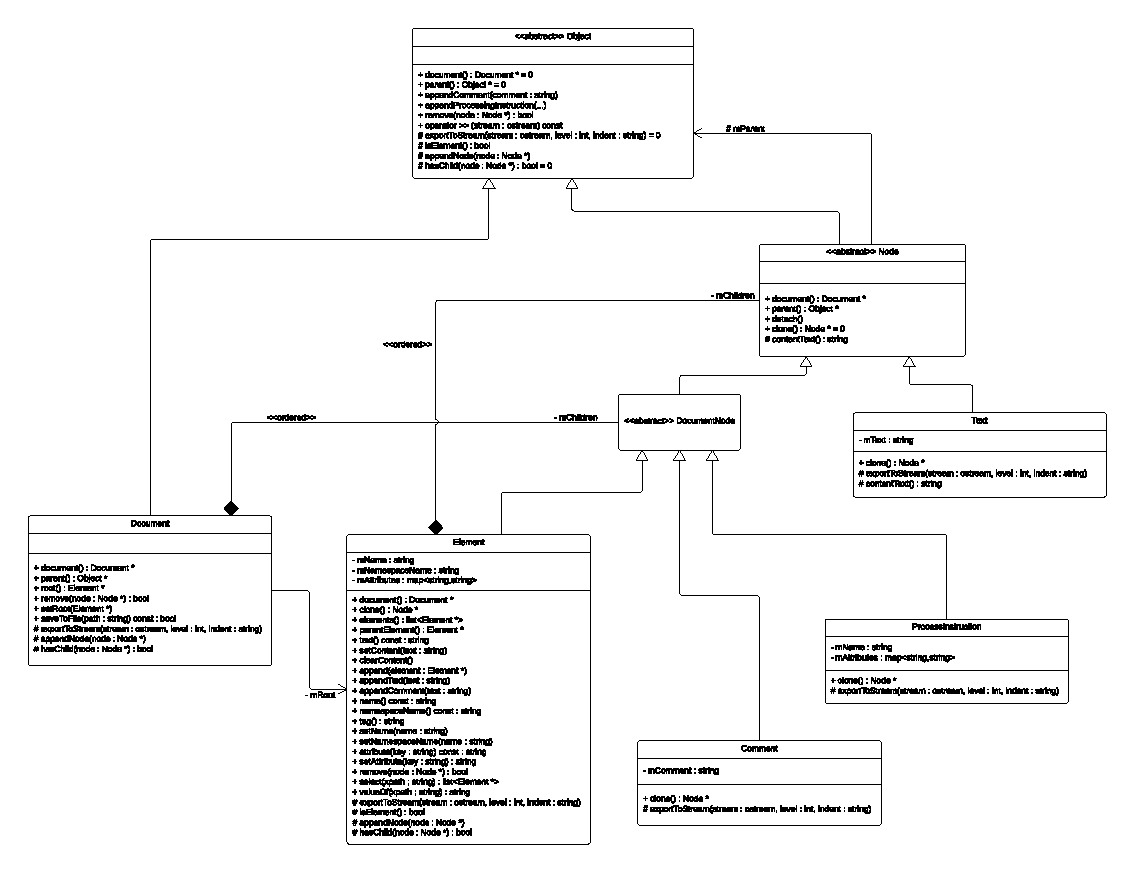
\includegraphics[width=0.9\linewidth]{images/xml-uml.pdf}
        \caption{Diagramme de classes de l'arborescence XML}
        \label{classDiagram}
    \end{figure}
    \end{landscape}


\section{Classes}
    \subsection{Log}
        La class \lstinline$Log$ a pour unique mission de stocker l'ensemble de l'output du parseur \textit{XML} telle que~:

        \begin{itemize}
            \item Erreurs lexicales~;
            \item Erreurs syntaxique~;
            \item Erreurs semantiques.
        \end{itemize}

    \subsection{Object}
        Pour optimiser et eviter au maximum la redondance de donner dans notre arbre d'h\'eritage de l'implementation \textit{XML}, nous nous somme inspirer de la tres c\'elebre librarie \textit{Qt} avec sont \lstinline$QObject$. Ainsi nous avons notre \lstinline$Xml::Object$ offrant les avantages que vous trouverez dans les sous sections suivantes.

    \subsection{Node}
        Ainsi, nous partons du principe qu'un document XML n'est en faite qu'un arbre aillant des noeux (\lstinline$Node$) \'etant des objects XML, mais de natures differents (commentaires, text, element ...). Certains de ces noeux serons des feuilles de l'arbre pour le noeux de commentaire par exemple.

        C'est la d\'ej\`a un avantage du \lstinline$Xml::Object$ car chaque \lstinline$Node$ connais sont \lstinline$Object$ parent \'a l'aide de \lstinline$mParent$ pouvant etre un \lstinline$Element$ ou un \lstinline$Document$. Ainsi, on peut \'a partir d'un noeud, retrouver le \lstinline$Document$ dans lequel il se trouve simplement en remontant l'arbre.

    \subsection{DocumentNode}
        Le \lstinline$DocumentNode$ est une sp\'ecialisation de \lstinline$Node$, mais aillant seulement une particularit\'e' s\'emantique~: seul ses classes fillent peuvent avoir pour parent, un \lstinline$Element$ par hertiage de \lstinline$Node$, mais aussi un \lstinline$Document$ au contraire de la classe \lstinline$Text$ ne pouvant avoir pour parent qu'un \lstinline$Element$.

    \subsection{Document}
        Un \lstinline$Document$ est un \lstinline$Node$ aillant une composition de \lstinline$DocumentNode$. Parmis ces \lstinline$DocumentNode$, un seul et unique \lstinline$Element$ racine compose cette liste. Mais afin de pouvoir retrouver cette racine du document en complexit\'ee $O(1)$, \lstinline$DocumentNode$ dispose aussi d'un attributs \lstinline$mRoot$ dedi\'e \`a cette tache.

        Cette m\^eme liste de \lstinline$DocumentNode$ est ordonn\'ee pour pouvoir garentir l'ordre des noeux au chargement et \`a l'export du document \textit{XML}. L'\lstinline$Element$ racine compose cette liste pour eviter de gerer deux listes de noeux (ceux avant et ceux apr\`es).

    \subsection{Comment}
        \lstinline$Comment$ est un \lstinline$DocumentNode$ car il peut \^etre n'importe ou dans le document \textit{XML}~: dans un \lstinline$Element$ ou bien en dehors de l'element racine du document.

    \subsection{ProcessingInstruction}
        Une \lstinline$ProcessingInstruction$ est aussi un \lstinline$DocumentNode$ d'apr\'es les specifications officiel de \textit{XML}. Mais en accord avec l'hypothèse énoncée précédemment, une \lstinline$ProcessingInstruction$ ne contient qu'un nom et une map d'attributs.

    \subsection{Text}
        Un noeud de texte est naturellement décrit par une chaîne de caractères \lstinline$mText$. Celui-ci ne dérive pas de la classe \lstinline$DocumentNode$ puisque, si son contenu s'apparente à celui d'un noeud Comment, il ne peut en revanche être contenu par une instance de \lstinline$Element$. D'ou la nécessit\'ee d'ajouter le niveau de spécialisation \lstinline$DocumentNode$ afin d'éviter une relation ne respectant pas les sp\'ecifications standart \textit{XML}.

    \subsection{Element}
        Un \lstinline$Element$ \textit{XML} est un \lstinline$DocumentNode$ car il poss\`ede une liste d'\lstinline$Element$ enfant \lstinline$mChildren$, mais aussi peut l'\lstinline$Element$ racine d'un \lstinline$Document$.

        Celui ci est defini avec un nom de balise (\lstinline$mName$) mais aussi d'un espace de nom (\lstinline$mNamespaceName$). La concatenation de ces deux derniers forme le tag de l'\lstinline$Element$. Le nom du membre \lstinline$mNamespaceName$ au lieu de \lstinline$mNamespace$ a \'et\'e effectuer pour eviter la colision avec le mot clef du language C++ \lstinline$namespace$ avec son getter th\'eorique \lstinline$Xml::Element::namespace()$ remplacer par \lstinline$Xml::Element::namespaceName()$.

        Un \lstinline$Element$ possede un ensemble non-ordonné d'attributs etant simplement une map aillant une assossiation $clef \leftarrow valeur$, par soucis de determinisme, nous les exportons par ordre alphabetique des clefs.

    \section{Algorithmes}

    \subsection{Xml::Element::select}

    \textbf{std::list<Xml::Element const *> Xml::Element::select(std::string const & xPathQuery);}

    \subsection{Xml::Element::valueOf}

    \textbf{std::string Xml::Element::valueOf(std::string const & xPathQuery);}

    \subsection{Xml::Element::matches}

    \textbf{bool Xml::Element::matches(std::string const & xPathQuery);}


	\chapter{XSD}

Dans cette partie, nous expliquerons notre conception de la partie validation d'un document XML à partir d'un document XSD.

\section{Hypothèses simplificatrices}
	Afin de simplifier l'implémentation du parseur XSD, les hypothèses suivantes ont été posées :
	\begin{itemize}
		\item{Les types simple seront de type \textit{string} ou \textit{date}}
		\item{Les types complexes seront de type \textit{sequence} ou \textit{choice} et pourront contenir des attributs}
	\end{itemize}
	
\section{Fonctionalités implémentées}
Les points suivants sont pris en charge par le validateur XSD :
\begin{itemize}
    \item{Choix d'éléments racine multiples}
    \item{Présence et type des attributs}
    \item{Éléments de types \textit{mixed}}
    \item{Types complexes contenant des éléments \textit{sequence} et \textit{choice} imbriqués}
    \item{Nombre d'occurences minimum et maximum par élément}
    \item{Références sur des attributs, éléments et types}
\end{itemize}

\section{Diagramme de classes}
Les classes ici décrites seront rattachées au \textit{\lstinline$namespace Xsd$} défini en C++.

\begin{landscape}
\begin{figure}[H]
	\centering
	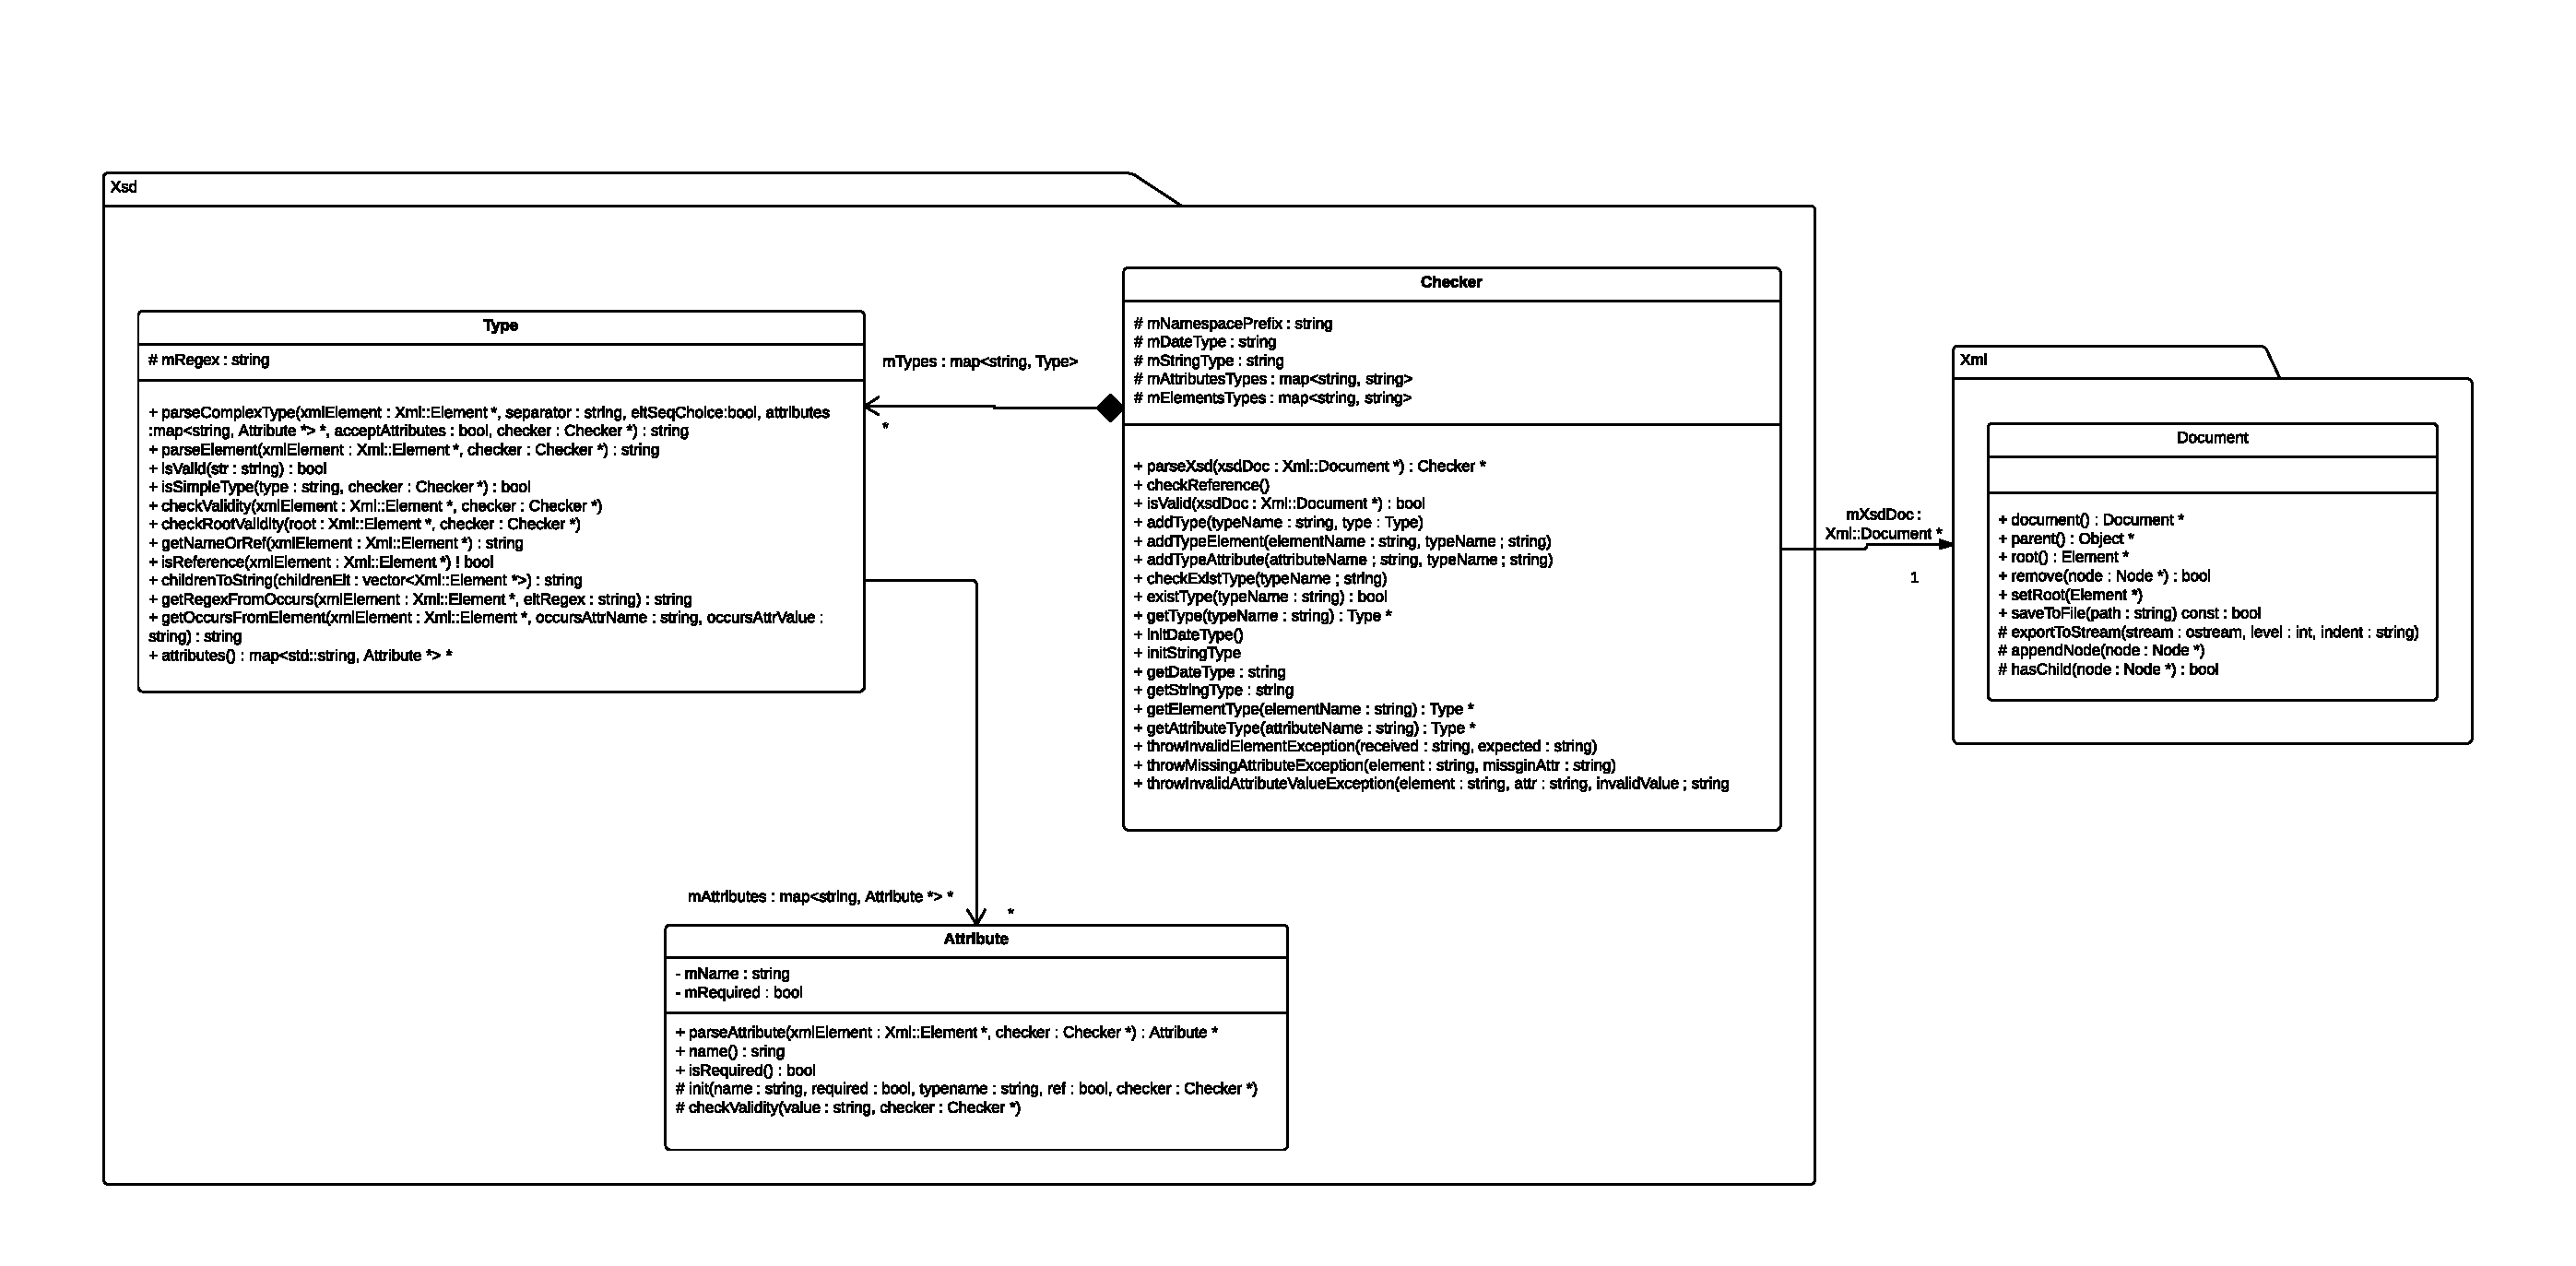
\includegraphics[width=\linewidth]{images/xsd-uml.pdf}
	\caption{Diagramme de classe de la validation xsd}
	\label{xsdClassDiagram}
\end{figure}
\end{landscape}

\section{Entités}
	\subsection{Checker}
		Un objet Checker décrit les règles présentes dans un document XSD. Les méthodes principales sont les suivantes :
		\begin{itemize}
			\item \textbf{parseXsd} : méthode statique retournant un objet de type \textit{Checker},  construit à partir du document XSD passé en paramètre
			\item \textbf{isValid} : retourne \textit{true} si le document XML passé en paramètre est en accord avec les contraintes inscrites dans l'objet \textit{Checker} courant, \textit{false} sinon
		\end{itemize}
		
		La structure intermédiaire s'appuie sur 3 tables de hachages :
		\begin{itemize}
			\item \textbf{mTypes} : associe le nom (chaîne de caractères) d'un type avec son objet de type \textit{Type}
			\item \textbf{mElementsTypes} : associe le nom d'un élément avec le nom de son type
			\item \textbf{mAttributesTypes} : associe l nom d'un attribut avec le nom de son type
		\end{itemize}
		
	\subsection{Element}
		Un élément est une chaîne de caractères, associé\footnote{Dans la suite de cette partie, le terme \textit{associer} correspondra à l'insertion d'une paire clé/valeur dans une table de hachage} à un type dans la table de hachage \textit{mElementsTypes} d'un objet de type \textit{Checker}.

	\subsection{Type}
		On objet \textit{Type} correspond à un type complexe XSD. Il est défini par deux éléments :
		\textit{Expression régulière} : Cette chaîne de caractères détermine l'ensemble des fils directs que l'élément rattaché au type peut recevoir. Elle spécifie leur ordre et nombre d'occurences.
			\textbf{Exemple} : \textit{(<fromage>){4}|(<poisson>){1})} sera l'expression régulière du type associé à l'élément \textit{pizza}.
			Elle indique qu'une pizza peut contenir 4 fromages ou un poisson.
		\textit{Liste d'attributs} : Cette liste décrit les attributs que contiendra l'élément rattaché au type courant, l'ordre des attributs n'ayant pas d'importance.
		
	\subsection{Attribute}
		Un attribut est décrit par son nom et un attribut \textit{required} à \textit{true} ou \textit{false}. Il est également associé à un type dans la table de hachage \textit{mAttributesTypes}.

\section{Algorithme}

\subsection{Construction de la structure intermédiaire}
L'algorithme présent construit un objet Checker, lequel contiendra un ensemble de types et attributs.
Cet algorithme parcours en une passe l'arbre XML obtenu lors du parsing préalable du document XSD.
Il s'agît d'un algorithme récursif, le parcours de l'arbre XML pouvant être assimilé à un parseur de type SAX sur le document XSD.

	\subsubsection{Parsing du document XSD : \textit{parseXsd}}
		\textbf{
		\lstinline$Parsing du document XSD sous forme d arbre XML$\\
		\lstinline$Parsing du type de l element racine (c.f. parseComplexType)$\\ \footnote{L élément \textit{schema} est implicitement de type complexe, ses éléments fils sont traités comme s ils étaient dans un élément \textit{choice}}
		\lstinline$Association du "ROOT_TYPE" avec le type reçu$\\
		\lstinline$Association du nom d element "ROOT" avec le type reçu$\\
		\lstinline$Verification des references (c.f. checkReferences)$\\

	\subsubsection{Parsing d'un élément \textit{complexType} : \textit{parseComplexType}}
		\lstinline$SI l element complexType a un attribut mixed a true$\\
		\indent \lstinline$Ajout de ".*" au separateur d elements de la regex$\\
					
		\lstinline$Parcours des fils de l element complextype$\\
		\indent \lstinline$SI c est un element sequence$\\
		\indent \lstinline \lstinline$Appel recursif$\\
		\indent \lstinline$SI c est un element choice$\\
		\indent \lstinline \lstinline$Appel recursif avec le separateur "|"$\\
		\indent \lstinline$SI c est un element element$\\
		\indent \lstinline \lstinline$on ajoute a la regex de l element complexType celle de l element retournee par parseElement() + le separateur$\\
		\indent \lstinline$SI c est un element attribute$\\
		\indent \lstinline \lstinline$Parsing de l attribut (c.f. parseAttribute)$\\
		\indent \lstinline \lstinline$Ajout de l attribut a la map d attributs du type courant$\\
						
		\lstinline$On retourne la regex associee au type$\\
				

	\subsubsection{Parsing d'un élément \textit{element} XSD : \textit{parseElement}}
		\lstinline$Construction d une regex decrivant l element en fonction de ses occurences$\\ \footnote{Par exemple, pour <xsd:element name="parfum" type="xsd:string" minOccurs="1" maxOccurs="2"/> on generera l expression (<pizza>){1}((<pizza>)?){1}}
		\lstinline$SI ce n est pas une reference$\\
		\indent \lstinline$SI l element a des enfants (c est un type complexe)$\\
		\indent \lstinline \lstinline$Construction d un type avec le premier fils de l element$\\ \footnote{Le constructeur de type appelle \textit{parseComplexType}}
		\indent \lstinline$Association du nom du type avec le type construit$\\
		\indent \lstinline$Association du nom de l element avec le nom du type construit$\\
					

	\subsubsection{Parsing d'un élément \textit{attribute} : \textit{parseAttribute}}
		\lstinline$SI les attributs nom et type sont definis, et que c est un type simple$\\
		\indent \lstinline$Association du nom de l attribut avec le nom du type$\\
		\lstinline$On retourne un nouvel attribut a partir d un nom et d un booleen required$\\
		}

	\subsubsection{Vérification des références : \textit{checkReferences}}
		\lstinline$Pour chaque element$\\
		\indent \lstinline$On verifie que l element est rattache a un type dans mElementsTypes$\\
		\lstinline$Pour chaque type$\\
		\indent \lstinline$Pour chaque attribut du type$\\
		\indent \indent \lstinline$On verifie que l attribut est rattache a un type dans mAttributesTypes$\\

\pagebreak

\subsection{Validation d'un document XML}
	\subsubsection{Validation d'un type : \textit{checkValidity}}
		Cette méthode prend un élément XML en paramètre, et valide les attributs qu'il contient et l'architecture de ses fils directs.
		L'appel initial est donc fait sur le type associé au nom de l élément root XML
		
		\lstinline$On verifie que l ensemble des attributs de l element XML existent dans la map des attributs du type XSD$\\
		\lstinline$Pour chaque attribut XSD du type XSD$\\
		\indent \lstinline$Si l attribut XSD existe$\\
		\indent \indent \lstinline$On verifie que sa valeur valide l expression reguliere de son type$\\
		\indent \lstinline$Si l attribut XSD n existe pas$\\
		\indent \indent \lstinline$On verifie qu il n est pas requis$\\
		
		\lstinline$Generation d une chaine de caracteres correspondant a la concatenation des balises de ses elements fils$\\
		\lstinline$On verifie que l expression reguliere du type valide cette chaîne de caracteres$\\
		
		\lstinline$Pour chaque element fils de l element XML reçu$\\
		\indent \lstinline$Recuperation du type associe au nom du fils$\\
		\indent \lstinline$Appel recursif a la fonction checkValidity sur le type obtenu$\\
		

	\chapter{XSL}

\section{Conception}

Dans un premier temps, nous avions choisi de suivre une conception orientée objet, et c'est donc
naturellement que nous avons proposé une classe dédiée aux documents \textit{XSL}, proposant les
fonctionnalités de transformation d'une feuille XSL, et de même pour les instructions \textit{XSL}.

\begin{figure}[h!]
    \centering
    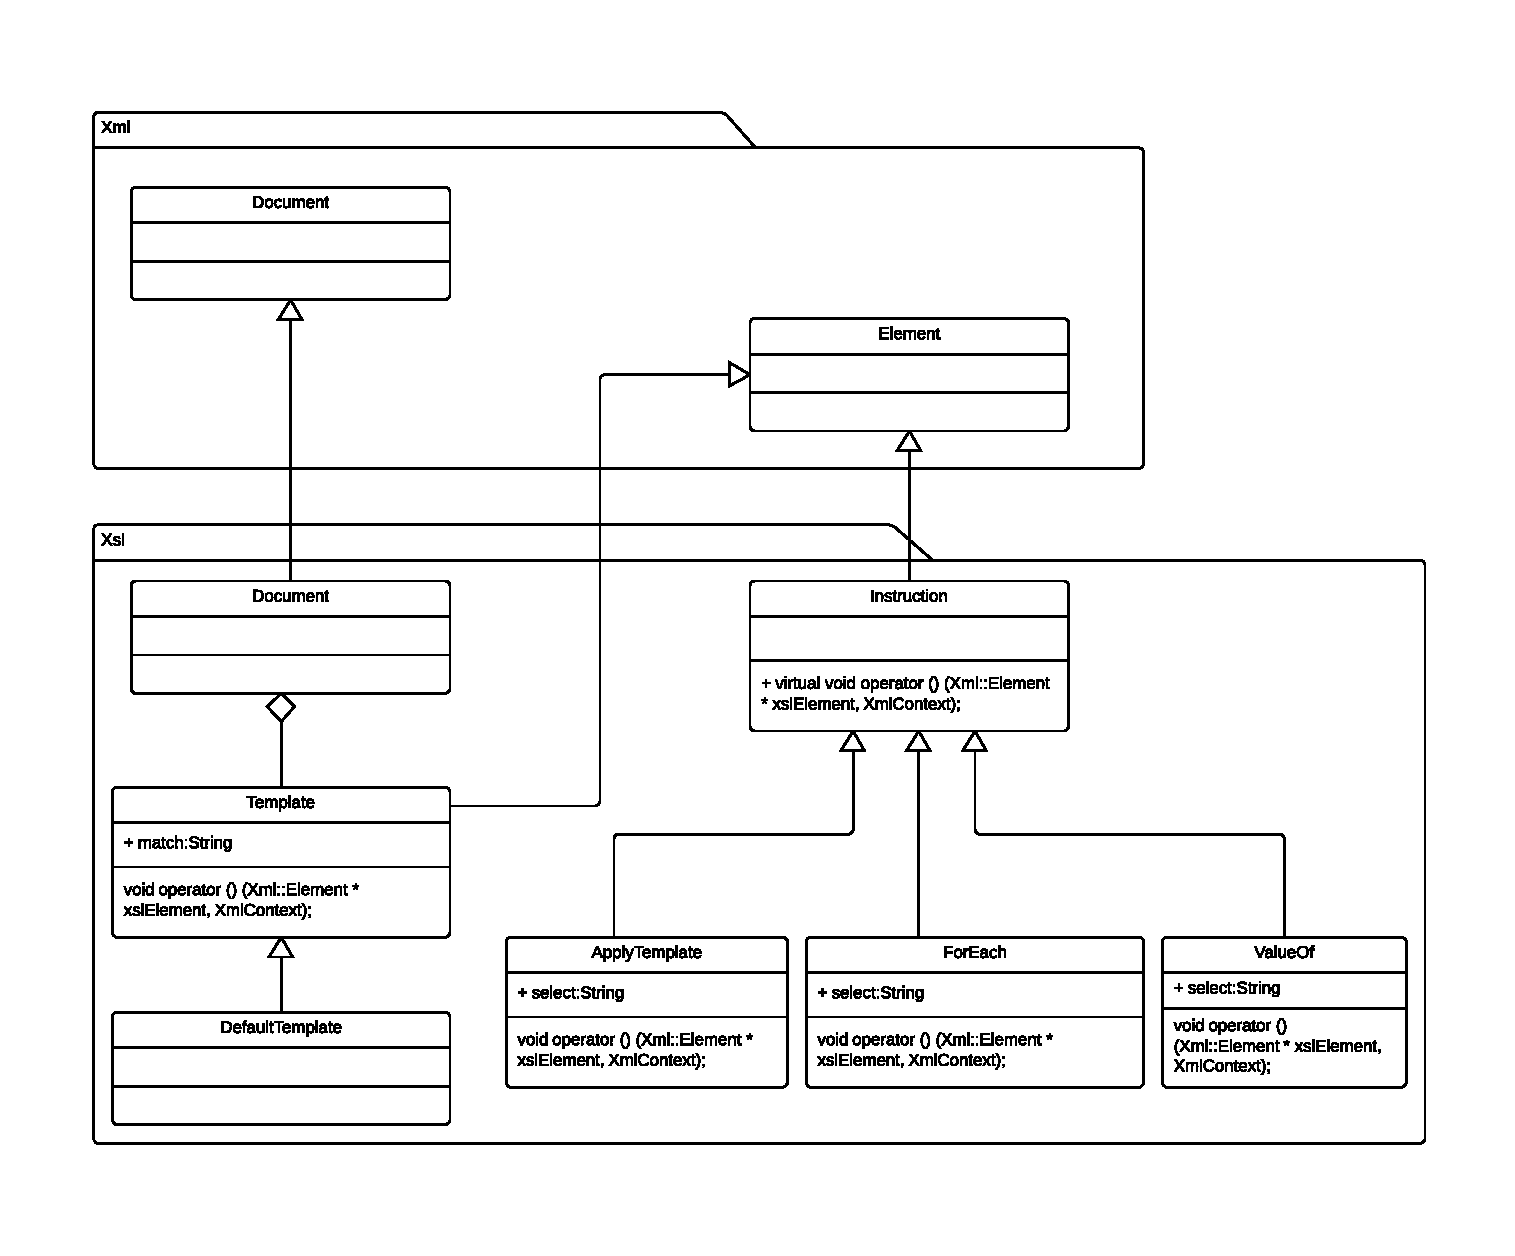
\includegraphics[width=\linewidth]{images/xsl-uml-old.pdf}
    \caption{Ancienne conception du module XSL}
    \label{oldXslClassDiagram}
\end{figure}

Néanmoins, cette conception présente de nombreux inconvénients : Elle nous forçait à parcourir tout le document XML afin de convertir les tags XSL en objets dédiés, ...

\textbf{TODO : } rajouter d'autres raisons pour lesquelles l'ancienne conception est pas pratique

\begin{landscape}
\begin{figure}[h!]
    \centering
    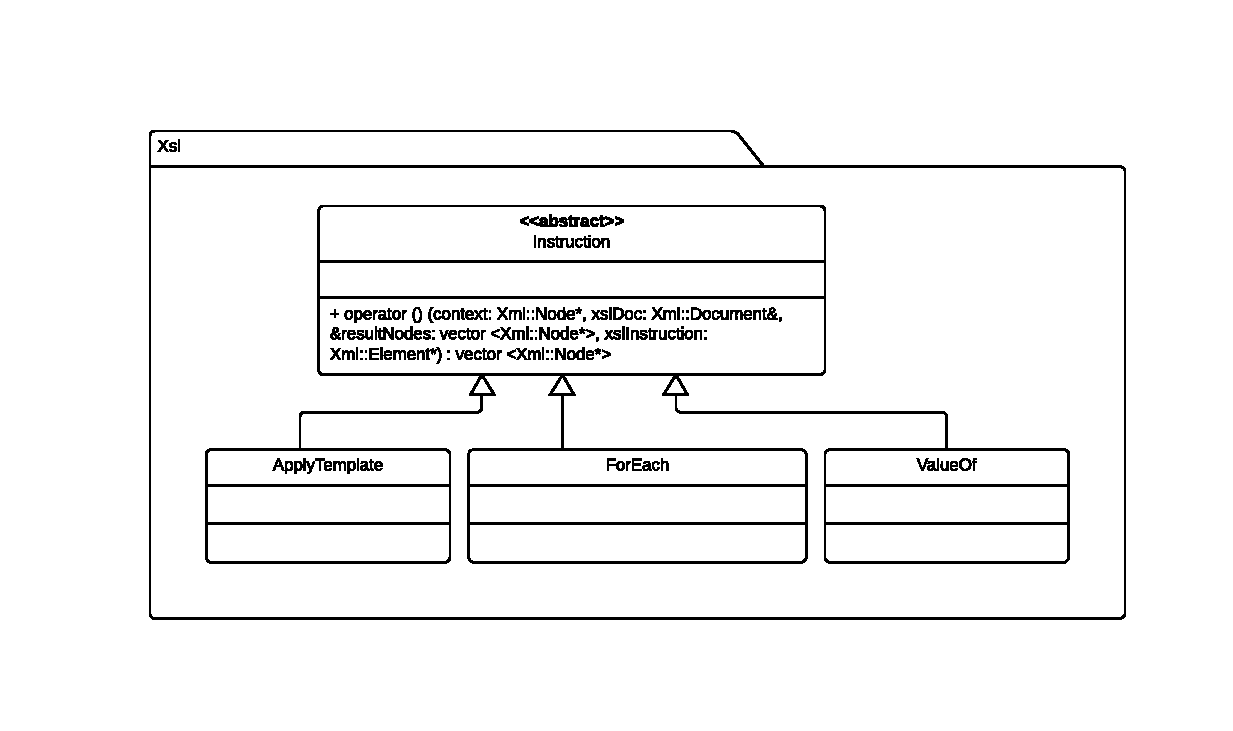
\includegraphics[width=\linewidth]{images/xsl-uml.pdf}
    \caption{Diagramme de classe des instructions XSL}
    \label{xslClassDiagram}
\end{figure}
\end{landscape}


\section{Vue globale de l'algorithme}

\textbf{TODO :} rajouter des détails sur cette partie.

L'algorithme de transformation XSL s’exécute de manière récursive et bascule continuellement entre le document XSL et le document XML à transformer.

Un même algorithme s'exécute pour chaque nœud (à quelques exceptions citées ci-dessous) :

\begin{enumerate}
    \item Si le nœud n'est pas un élément, on le rajoute directement au résultat.
    \item Si un \textit{template} correspond à ce nœud, on l'applique (plus sur l'application des templates ci-dessous) en prenant ce nœud comme \textit{contexte} et on ajoute le résultat de cette application au nœud contexte.
    \item Sinon, on clone l'élément, et on ré-applique le même algorithme sur tous ses enfants, en ayant comme contexte le nœud qu'on a cloné et en rajoutant tous les résultats comme fils du clone du nœud.
\end{enumerate}

La transformation XSL débute en appliquant cet algorithme à la racine du document XML à transformer, et se propage par récursion à la totalité du document.


\section{Templates}

Les \textit{templates} sont les seuls fils de la racine (\textit{stylesheet}) d'un document XSL et se présentent de la manière suivante :
\\
\\
\textbf{
\lstinline$<xsl:template match="cd/title">$\\
\indent \lstinline$<tagxml></tagxml>$\\
\indent \lstinline$<xsl:uneinstruction select="untag/unautretag" />$\\
\indent \lstinline$<encoreunautretagxml />$\\
\lstinline$</xsl:template>$
}
\\
\\
Ils peuvent contenir des tags XML "normaux", ainsi que des instructions XSL.
On dit qu'un template \textit{match} un élément si l'élément est compatible avec la valeur de l'attribut \textit{match} du template, par exemple :

Si un élément XML a comme nom "title" et est le fils d'un élément qui a comme nom "cd", il match le template vu ci-dessus.

Quand on applique un template, on va renvoyer une liste de nœuds résultants (qui vont en général être ajoutés comme fils d'un document ou d'un élément). Cette liste est générée de la manière suivante :\\

\begin{enumerate}
    \item Les nœuds qui ne sont pas des éléments XML sont rajoutés directement.
    \item Les nœuds qui sont des éléments XML, mais pas XSL, sont considérés comme des templates (car pouvant contenir des instructions XSL) et appliqués avec comme contexte le nœud d'application de la transformation XSL.
    \item Les éléments XSL sont appliqués avec comme contexte le nœud d'application de la transformation XSL. Tous les nœuds résultants de cette application sont ajoutés à la liste des nœuds générés par l'application du template.

\end{enumerate}

	%\renewcommand{\chaptermark}[1]{\markboth{\MakeUppercase{#1}}{}}
	%\renewcommand{\sectionmark}[1]{\markright{#1}}

	%\addcontentsline{toc}{part}{Annexes}
	%\part*{Annexes}
	%\appendix
	%\include{implementationExercices}


    % ------------------------------------------------------------------- FOOTER
\end{document}
